

\chapter{Blocage de Coulomb}

Dans ce chapitre nous allons aborder le transport à travers une structure nanoscopique et nous allons nous intéresser en particulier au phénomène de blocage de Coulomb. Ce phénomène a d'abord été observé sur des échantillon métallique macroscopique composé de petit grain métallique par C.J. Gorter en 1951. En mesurant la conductance d'un de ces échantillon en fonction de la température, l'auteur a constaté une diminution inattendu à basse température. Cette diminution de la température à été attribué à l'aspect granuleux du métal. Plus précisément , pour ajouter un électron dans un des grains constituant le métal, il fallait fournir une énergie $e^2/C$ où $e$ est la charge de l'électron et $C$ est la capacité que l'on peut associé à un de ces grains. A haute température ($k_bT >> e^2/C$), cette énergie n'affecte pas la conductance du système. A basse température en revanche ($k_bT << e^2/C$), cette enérgie réduit l'habilité des électron à se mouvoir librement dans le métal ce qui entraîne une diminution de la conductance. Depuis, l'étude de ce phénomène à beaucoup évolué et de nos jours et le rôle central du grain de métal est souvent remplacé par des molécules, des point quantique de gaz d'électron à deux dimensions etc..

Dans ce chapitre, nous verrons tout d'abord qu'elles sont le différent paramètres physique d'un système type. En particulier, nous donnerons quelques conditions nécessaire à l'apparition d'un phénomène de blocage de Coulomb classique et quantique. Nous aborderons ensuite la notion de potentiel chimique et nous montrerons comment cette notion peut expliquer de façon intuitive le phénomène de blocage de Coulomb. Nous déterminerons notamment comment certain paramètre du système par une simple mesure de courant. Nous développerons ensuite un modèle plus quantitatif afin de déterminer le courant circulant à travers une structure nanoscopique. Pour cela, nous nous concentrerons sur le cas particulier d'une boite quantique oscillant entre deux états de charge.



\section{Les paramètres du système}
La description que nous proposons ici est celui d'un système à trois terminaux que l'on nommera la source, le drain et la grille, ainsi qu'un il\^ot dont la nature peut varier suivant les cas. On peut imaginer une molécule, un il\^ot métallique, un gaz d'électron deux dimensions etc.. L'il\^ot est couplé capacitivement au trois terminaux par trois capacitance ; $C_g$ pour la grille, $C_d$ pour le drain et $C_s$ pour la source. De plus, des barrière tunnel entre l'il\^ot et la source et l'il\^ot et le drain permettant le passage d'électron (sous certaines conditions). Ces deux barrières tunnels sont caractériser par les paramètre $\gamma_s$ pour le système source/il\^ot et $\gamma_d$ pour le système drain/il\^ot. La source et le drain sont considéré comme des matériaux massif métallique et dont les électrons obéisse à la statistique de Fermi-Dirac. Enfin, nous attribuons à l'il\^ot une taille caractéristique $L$. Tous ces paramètre sont représenté dans la Fig. \ref{description_systeme}. Nous allons maintenant regarder plus en détail chacun des ces paramètres.

\subsubsection{Les capacitances du système}
Comme expliqué précédemment, trois capacitances couples l'il\^ot central aux trois terminaux. De part ces capacitances, l'application d'un tension sur l'un ou plusieurs terminaux va modifier l'energie des électrons situés sur l'ilôt. Cette modification peut facilement s'exprimer comme suit :

\begin{eqnarray}
E = \frac{(C_sV_s + C_dV_d + C_gV_g)^2}{2(C_g + C_s + C_g)}=\frac{(C_sV_s + C_dV_d + C_gV_g)^2}{2C_{\Sigma}} \nonumber
\end{eqnarray}

De plus, ces capacitance vont induire un "co\^ut" énergétique à l'ajout d'un électron dans l'il\^ot central. L'ajout d'un électron est associé à l'énergie $\frac{E_c}{2}$~(nous verrons l'utilité du facteur un-demi dans la suite). Cette énergie est donné par :
\begin{eqnarray}
\frac{E_c}{2} = \frac{e^2}{2(C_s+C_d+C_g)}=\frac{e^2}{2C_{\Sigma}} \nonumber
\end{eqnarray}


Ces cette énergie qui est à l'origine de la diminution de la conductance observée par C.J. Gorter en 1951. On voit ici une première condition nécessaire à l'apparition du phénomène du blocage de Coulomb : $E_c >> k_bT$.

On peut donc exprimer l'énergie d'un il\^ot contenant N électrons et soumis à trois tensions $V_g$, $V_d$ et $V_s$ comme suit :
\begin{eqnarray}
U(N) = \frac{1}{2C_{\Sigma}} (-|e|N + C_sV_s + C_dV_d + C_gV_g)^2
\end{eqnarray}

\begin{figure}
\includegraphics[scale=1]{Theorie/Transport/figure1/figure1ThTr.pdf} 
\caption{Paramètres caractérisant un système à trois terminaux}
\label{description_systeme}
\end{figure}



\subsubsection{La taille de l'il\^ot}
Comme nous l'avons précisé précédemment, nous étudions des structure nanoscopique ou autrement dit $L\sim nm$. Pour de telle dimension, on observe une quantification des différent état du système il\^ot. Les spectre énergétique de l'il\^ot peut s'exprimer en fonction de trois nombre quantique $n_x$,$n_y$ et $n_z$ à travers la relation suivante:
\begin{eqnarray}
E_n = \frac{\pi^2 \hbar^2}{2m}(\frac{n_x^2}{L_x^2} + \frac{n_y^2}{L_y^2} + \frac{n_z^2}{L_z^2}) \nonumber
\end{eqnarray}


Il s'agit bien entendu ici d'une expression très simplifié. Dans le cas de molécules par exemple, cette quantification simpliste est remplacé par la quantification correspondante aux orbitale moléculaire. Pour résoudre expérimentalement cette quantifications des niveaux la condition $\frac{\pi^2 \hbar^2}{2mL} >> k_bT$. Le seul moyen d'action de l'expérimentateur se fait à la fois sur $L$ en diminuant la taille des objets observés et $T$ en utilisant des frigo à dilution. Lorsque cette condition est rempli, on rentre dans le régime du blocage de coulomb quantique.
\newline


\subsubsection{Les paramètre de couplage tunnel $\gamma_{s/d}$}
On peut voir ces coefficient comme définissannt la "facilité" avec laquelle les électrons peuvent passer par effect tunnel de la source ou du drain vers l'il\^ot et vice-versas. Les valeur $\gamma_{s/d}$ sont déterminante dans la valeur du courant qui va \^etre mesuré dans notre système. De plus, le couplage à la source et au drain contribue à l'élargissement des niveaux d'énergie d'une largeur $\Delta E$ donnée par :
\begin{eqnarray}
\Delta E_{\text{intrinsèque}} = h (\gamma_s + \gamma_d)
\end{eqnarray}
Cette élargissement est appelé élargissement intrinsèque par opposition à l'élargissement induit par la température. On peut deviner ici une seconde condition nécéssaire à l'apparition du phénomène de blocage de Coulomb à savoir $\Delta E_{\text{intrinsèque}} << E_c$. De plus, dans un régime de blocage fort on a $\Delta E_{\text{intrinsèque}} << k_bT$. Si cette dernière condition est remplie, on peut donc avoir accès par l'intermédiaire de des distribution de Fermi-Dirac à la température du système. C'est cette propriété qui est utilisé dans le thermomètre à blocage de Coulomb.





\section{La notion de potentiel chimique}
La notion de potentiel chimique est à mes yeux une des notions les plus importantes afin de comprendre de manière simple et intuitive le phénomène de blocage de Coulomb. Un exemple de son utilisation dans la cadre du transport quantique peut \^etre trouvé dans la très belle et très pédagogique revue de Hanson \textit{et Al.}. Dans cette section, nous allons tout d'abord présenté le concept de potentiel chimique. Nous exprimerons ensuite, à partir des considération exposé dans la partie précédente, le potentiel chimique de la source, du drain et surtout de l'ilôt central.

\subsubsection{Définition}

On recontre souvent le potentiel chimique en thermodynamique lorsque l'on s'intéresse aux systèmes ouvert échangeant des particules. Cette grandeur défini la variation d'énergie d'un système du à la modification du nombre de particule qui le compose. On le trouve parfois défini comme suit :
\begin{eqnarray}
\mu = \frac{\partial U}{\partial N} \nonumber
\end{eqnarray}
$U$ étant l'énergie du système et $N$ le nombre de particule. Dans la suite, nous allons plut\^ot adopter la notation de Hanson et Al. et prendre la définition suivante :
\begin{eqnarray}
\mu(N) = U(N) - U(N-1)
\end{eqnarray}
ou $\mu(N)$ est la modification en énergie apporté par l'ajout de la $N^\text{nième}$ particules, $U(N)$ et $U(N-1)$ étant respectivement l'énergie du système avec $N$ et $N-1$ particules.

Maintenant, partant de cette définition on peut imaginer un système de trois réservoirs. Supposons maintenant que l'on puisse atribuer à chacun des ces réservoirs un potentiel chimique et que deux plus, ces potentiels chimiques soient alignés. Je nommerai ces potentiel chimique $\mu_{droit}$, $\mu_{centre}$ et $\mu_{gauche}$. On a donc $\mu_{droit}=\mu_{centre}=\mu_{gauche}$.

Si maintenant je prends une particule dans le réservoir de droite et que je là mets au centre. L'énergie du réservoir de droite va varié de $-\mu_{droit}$ tandis que l'énergie du réservoir du centre va varier de $\mu_{centre}$. En revanche la variation totale en énergie du système est nulle. 

En faisant de m\^eme avec le réservoir de gauche, on arrive à la conclusion que les trois configuration ; la particule à droite au centre ou à gauche ont la m\^eme énergie ou autrement dit, sont dégénéré. Nous verrons dans la suite que une telle configuration sera appelé point de dégénérescence. 

De fait, la particule est libre de circuler d'un point du système à l'autre. Nous voyons donc que la notion de potentiel chimique nous permet d'identifier ou non la possibilité pour des particules de passer d'un réservoir à l'autre en fonction du potentiel chimique qui leur est associés. Nous utiliserons cette propriété dans la suite pour définir les contitions de circulation d'électron dans notre système. Mais pour cela, il faut définir ce qu'est le potentiel chimique dans le cas de nos trois réservoir à savoir: la source, le drain et bien sûr l'ilôt.


\subsubsection{Les potentiels chimique de la source et du drain.}
L'expression du potentiel chimique de la source et du drain est directement donnée par $\mu_i = e V_i$ ou $i=source/drain$. Il s'agit en fait du niveau de Fermi des électron dans la source et le drain (à ne pas confondre avec l'énergie de Fermi). Si l'on veut maintenant savoir quel est la probabilité dans un métal de niveau de fermi $\mu_F$ de trouvé un électron de potentiel chimique $\mu$, je peux utiliser la distribution de fermi et cette probabilité est donc égale à :
\begin{eqnarray}
p(\mu) = \frac{1}{1 + \exp{(\frac{\mu - \mu_F}{k_bT})}} \nonumber
\end{eqnarray}
 On obtient donc en fonction des tensions source et drain:
\begin{eqnarray}
p_i(\mu) = \frac{1}{1 + \exp{(\frac{\mu - eV_i}{k_bT})}}
\end{eqnarray}
ou $i=source/drain$. Nous verrons dans la suite que cette notion est essentielle dans la détermination du courant qui traverse notre structure.

\begin{figure}
\centering 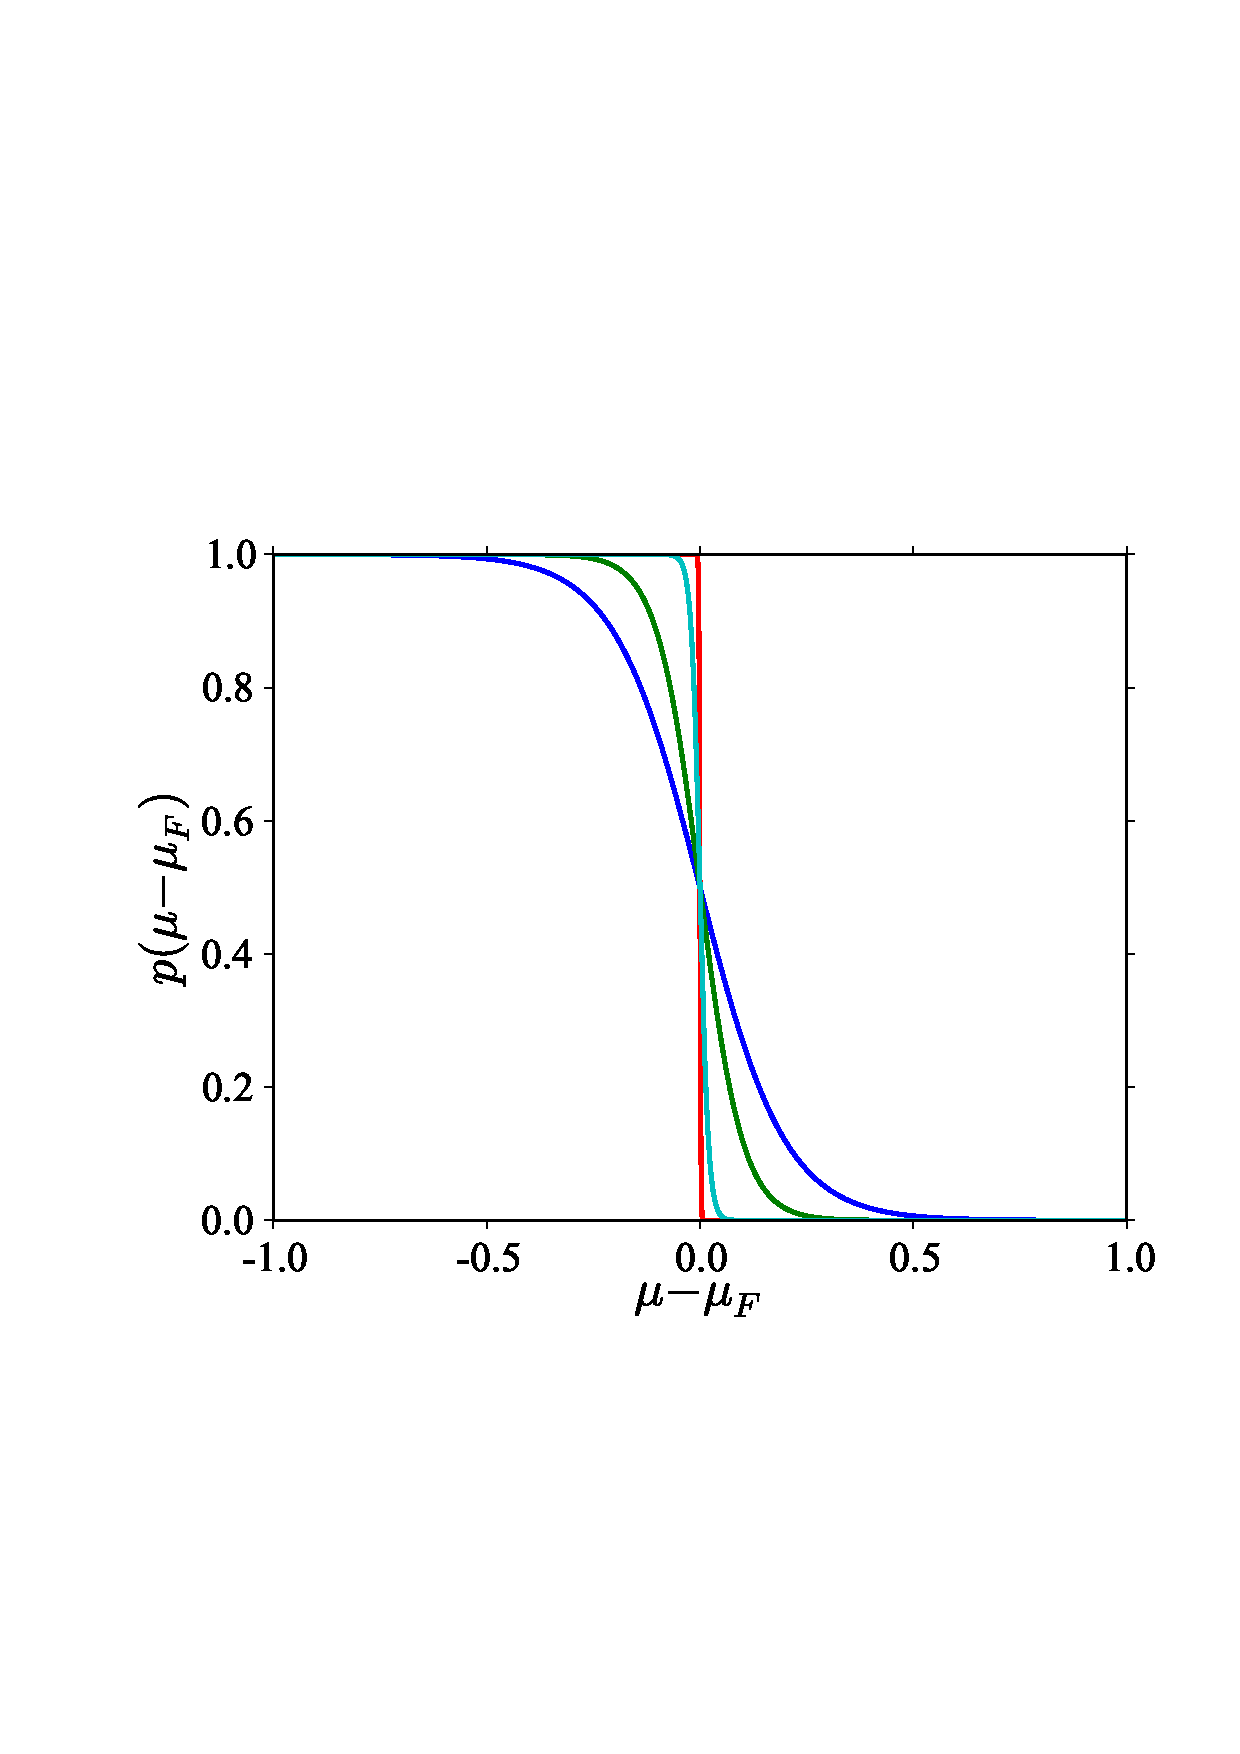
\includegraphics[scale=0.5]{Theorie/Transport/figure2/figure2.pdf} 
\caption{Probabilité d'avoir un électron de potentiel chimique $\mu$ sachant que le potentiel chimique du métal est $\mu_{\rm{F}}$. Le potentiel chimique $\mu_{\rm{F}}$ correspondant à une tension de $1mV$ que l'on applique habituellement dans ce genre d'éxpérience correspond à une énergie de $11.5K$.}
\label{distrib_fermi}
\end{figure}



\subsubsection{Le potentiel chimique de l'il\^ot}
Si l'expression du potentiel chimique de la source et du drain n'a rien de compliqué (dans le cas d'életrode normale tout du moins), on ne peut pas en dire de m\^eme de celle de l'il\^ot. C'est m\^eme là que réside toute la difficulté de la compréhension d'une expérience. Heureusement, dans la partie précédente nous avons déjà fait le bilan des différentes énergie en jeux dans le système. A savoir, nous devons prendre en compte l'énergie électrostatique du système, l'énergie d'interaction électron-électron ainsi que la discrétisation des niveaux d'énergie dans l'il\^ot. Tout ceci donne :
\begin{eqnarray}
U(N) = \underbrace{\frac{1}{2C_{\Sigma}} (-|e|N + C_sV_s + C_dV_d + C_gV_g)^2}_{\text{couplage électrostatique et énergie de charge}}
+ 
\underbrace{\sum_{n=1}^{N} E_n}_{\substack{\text{énergie liés aux} \\\text{aux états discret}}}
\end{eqnarray}
On peut également tenir compte d'un éventuel champ magnétique en faisant le remplacement suivant :
\begin{eqnarray}
\sum_{n=1}^N E_n = \sum_{n=1}^N E_n(B) \nonumber
\end{eqnarray}
c'est à dire en attribuant à chaque niveau discret, une dépendance en champ magnétique. Nous verrons rapidement dans la suite comment cela se traduit dans le cas d'un système simple. 

Une fois l'énergie en fonction de $N$ exprimer simplement, il suffit d'appliquer la définition précédente à savoir :
\begin{eqnarray}
\mu(N) = U(N) - U(N-1) \nonumber
\end{eqnarray}
On se retrouve avec une expression relativement simple du potentiel chimique :
\begin{eqnarray}
\mu(N) = (N-\frac{1}{2})\frac{e^2}{C_{\Sigma}}
+ 
\frac{e}{C_{\Sigma}}(C_gV_g + C_sV_s + C_dV_d)
+
E_N(B)
\end{eqnarray}

Si maintenant, on se rappelle que nous avons défini plus haut l'énergie de charge $\frac{E_c}{2} = \frac{e^2}{C_{\Sigma}}$, nous pouvons réécrire la relation précédente sous la forme :

\begin{eqnarray}
\mu(N) = (N-\frac{1}{2})E_c
- 
\frac{E_c}{|e|}(C_gV_g + C_sV_s + C_dV_d)
+
E_N(B)
\label{pot_chim}
\end{eqnarray}
L'énergie $E_c$ est donc la quantité d'énergie d\^u à la répulsion Coulombienne qui sépare deux potentiels chimiques d'état de charge différents.


\section{Détermination des conditions de circulation d'un courant}
Pour rendre l'exposé qui va suivre plus clair, nous allons le décomposé en trois partie. Dans la première partie, nous allons voir quelles sont les conditions à remplir pour qu'un électron du drain puisse aller dans l'il\^ot. Dans la deuxième partie, nous ferrons de m\^eme pour la source. Enfin, dans la dernière partie, nous exploiterons les résultats obtenues pour en déduire les conditions pour qu'un courant circule dans notre structure ainsi que le signe de ce courant en fonction des paramètres. Afin d'adapter les solutions trouvées au condition expérimentale, on posera $V_s = 0$ car dans la grande majorité des dispositif, une des électrodes est directement connecter à la masse. Ce qui donnera $V_d=V_{ds}$, $V_{ds}$ étant la tension appliqué à l'échantillon au traver de la source et du drain.

\subsubsection{Charge de l'il\^ot par le drain}
Comme nous en avons discuté précédemment, pour qu'un particule (ici un électron) puisse passer d'un réservoir à l'autre, il faut que son potentiel chimique soit identique dans les deux réservoirs. Si l'on adapte se raisonnement à notre système, il faut donc qu'il y ait dans le drain des électrons dont le potentiel chimique corresponde à celui de cette électron une fois sur l'il\^ot. Supposoent donc l'il\^ot dans l'état de charge $N-1$, pour passer à l'état de charge $N$, il faut qu'il y ait au moins un électron dont le potentiel chimique soit égale à $\mu(N)$. Il nous suffit d'oberver la courbe de la Fig. \ref{distrib_fermi} pour comprendre que cela suppose :
\begin{eqnarray}
-|e|V_{ds} \geq \mu(N)
\end{eqnarray}
Ce qui conduit à la relation suivante :
\begin{eqnarray}
-|e|V_{ds} \geq (N-\frac{1}{2})\frac{e^2}{C_{\Sigma}}
-
\frac{|e|}{C_{\Sigma}}(C_gV_g + C_sV_s + C_dV_d)
+
E_N(B) \nonumber
\end{eqnarray}
En se rappelant que $V_s= 0$ et que $V_{ds} = V_d$, on en déduit la relation suivante :
\begin{eqnarray}
V_{ds} \leq \frac{1}{C_{\Sigma}}(C_gV_g + C_dV_{ds}) + \frac{E_N(B)}{|e|} - (N-\frac{1}{2})\frac{|e|}{C_{\Sigma}} \nonumber
\end{eqnarray}
Cette relation peut se réécrire de la façon suivante :
\begin{eqnarray}
V_{ds} \leq \frac{1}{C_g + C_s} \{C_gV_g - \frac{C_{\Sigma}}{|e|}[E_N(B) + (N-\frac{1}{2})E_c] \}
\end{eqnarray}
De cette formule nous pouvons en déduire deux relations importantes. Comme on peut le voir, l'état de charge $N$ décale la droite caractéristique de charge de l'il\^ot. De cette constatation, on peut en déduire que la séparation en tension de grille $\Delta V_g$ et liée à l'énergie du système par :
\begin{eqnarray}
\frac{C_g}{C_{\Sigma}} |e| \Delta V_g = E_c + \Delta E
\end{eqnarray}
Le deuxième enseignement est que la zone de transition entre charge et décharge dans le plan ($V_g$,$V_{ds}$) est délimité par une droite dont la pente est donnée par les différentes capacitances du système. Cette pente est donnée par 
\begin{eqnarray}
\frac{C_g}{C_g + C_s}
\end{eqnarray}



\begin{figure}
\includegraphics[scale=0.5]{Theorie/Transport/figure3/figure3.pdf} 
\caption{Représentation de la charge et de la décharge de l'il\^ot dans le plan ($V_g$,$V_{ds}$)}
\label{charge_discharge}
\end{figure}



\subsubsection{Charge de l'il\^ot par la source}
Un raisonnement similaire au précédent et en se rappelant que $V_s = 0$ conduit à la relation suivante :

\begin{eqnarray}
V_{ds} \geq -\frac{1}{C_d} \{C_gV_g + \frac{C_{\Sigma}}{|e|}[E_N(B) + (N-\frac{1}{2})E_c] \}
\end{eqnarray}


On peut extraire une deuxième pente qui correspond à la charge ou la décharge de l'il\^ot par la source.


\subsubsection{Condition de circulation du courant}

Si l'on reprend les deux paragraphes précédent, on peut imaginer quatre situtation :
\begin{enumerate}
\item aucun électron ne peut \^etre chargé ni par la source ni par le drain. L'état de charge reste à N.
\item un électron peut \^etre chargé à la fois par la source et par le drain. Il va donc y demerer et l'état de charge est N+1.
\item un électron ne peut \^etre charge que par la source. Dans ce cas, il finit par se décharger dans le drain
\item un électron ne peut \^etre chargé que par le drain. Dans ce cas, il finit par se décharger dans la source.
\end{enumerate}
Dans les cas un et deux, l'état de charge de l'il\^ot est bien défini et on se trouve dans le régime de blocage de Coulomb. Dans le cas 3 les électrons circulent de la source vers le drain. Un courant positif est donc mesuré. Dans le cas 4, les électrons circulent du drain vers la source. Un courant négatif est donc mesuré. L'emsemble de ces régimes est représenté dans la Fig. \ref{charge_discharge}.










\section{Etats excités et transport}
Dans ce dernier paragraphe nous allons aborder la notion de spectroscopie par transport. Cette méthode vise à analyser les différents état du système par des mesures de transport. Cette technique à notablement été utilisé pour sonder les niveaux magnétique par l'application d'un champ et par l'étude de l'évolution des propriété de transport en fonction de ce champ magnétique.

Nous allons pour aborder cette technique, nous consacrer sur le système que nous avons décrit précédemment dans le cadre de l'équation pilote. Le diagramme Zeeman de l'état de charge N=1 est représenté avec les potentiels chimique associé à la transition 0/1.

A partir de ces potentiels chimique on peut déjà esquissé l'allure de la cartographie de conductance dans le plan ($V_g$,$V_{ds}$). Il suffit pour cela de tracer un double jeux de Diamant de Coulomb. On utilise ensuite les bord de Diamant correspondant à la transition état fondamental de l'état 0 à l'état fondamental de l'état de charge 1. Lorsque d'un bord de Diamant associé à un état excité, ce bord de Diamant doit \^etre stoppé et ne pas allé jusqu'à l'origine. On peut identifier deux zones de lecture pour ce qui est des états d'énergie : par la tension de grille en prolongeant les bords de diamant de Coulomb ou par la tension source drain. Dans les deux cas, une renormalisation de l'énergie est nécessaire.

Une approche plus qualitative peut \^etre obtenue en utilisant les équations pilotes et confirme ce que l'on avait obtenue avec la méthode plus simple des potentiels chimique. En revanche, la technique de l'équation pilote nous donne plus d'information sur l'amplitude des différentes variations de courants.

Ces deux marche successive en courant correspondent à l'entré dans la fen\^etre de tension $V_{ds}$ d'un puis de deux canaux correspondant respectivement à la transition état fondamental état fondamental et état fondamental excité. Dans des système plus complexe, ils arrivent souvent que les état N/N+1 possèdent tout deux des états fondamentaux et des états excités. Dans ce cas, la signature en transport devient plus complexe. Ces différentes configurations sont notamment traité par Hanson et Al., et un exemple peut \^etre trouvé dans l'analyse du $N@C_{60}$ proposé en fin de thèse et les références qu'il contient.

\begin{figure}
\includegraphics[scale=0.5]{Theorie/Transport/figure4/figure4.pdf} 
\caption{Diagramme Zeeman de l'état de charge N=1. Potentiel chimique correspondant à la transition 0/1}
\label{charge_discharge}
\end{figure}

On peut également une autre mesure qui prendra tout son sens dans la suite quand on utilisera l'il\^ot central non plus comme le système à étudier mais comme un sonde de son environnement local. Nous vennons de voir que la position du point de dégénérescence dépend de la position du potentiel chimique dans l'échelle des énergies. On peut donc choisir une tension de grille $V_g$ proche du point de dégénérescence avec une tension source-drain $V_{ds}$ nulle. On mesure en suite la conductance en faisant varier le champ magnétique.